\chapter{Communication in the Swarm}

\paragraph*{}
Swarm communication has been successfully implemented using socket-based communication within a peer-to-peer architecture. This approach was selected due to its reliability and low-latency performance, which are essential for real-time robotic coordination. Within the swarm, this communication framework enables robots to continuously exchange positional data, facilitating effective self-collision avoidance. Furthermore, it supports the transmission of relevant information to the designated taskmaster, thereby enabling the transition to the path planning phase. The primary communication flow is outlined below. (Figure \ref{fig:communication-flow})

\begin{figure}[H]
    \centering
    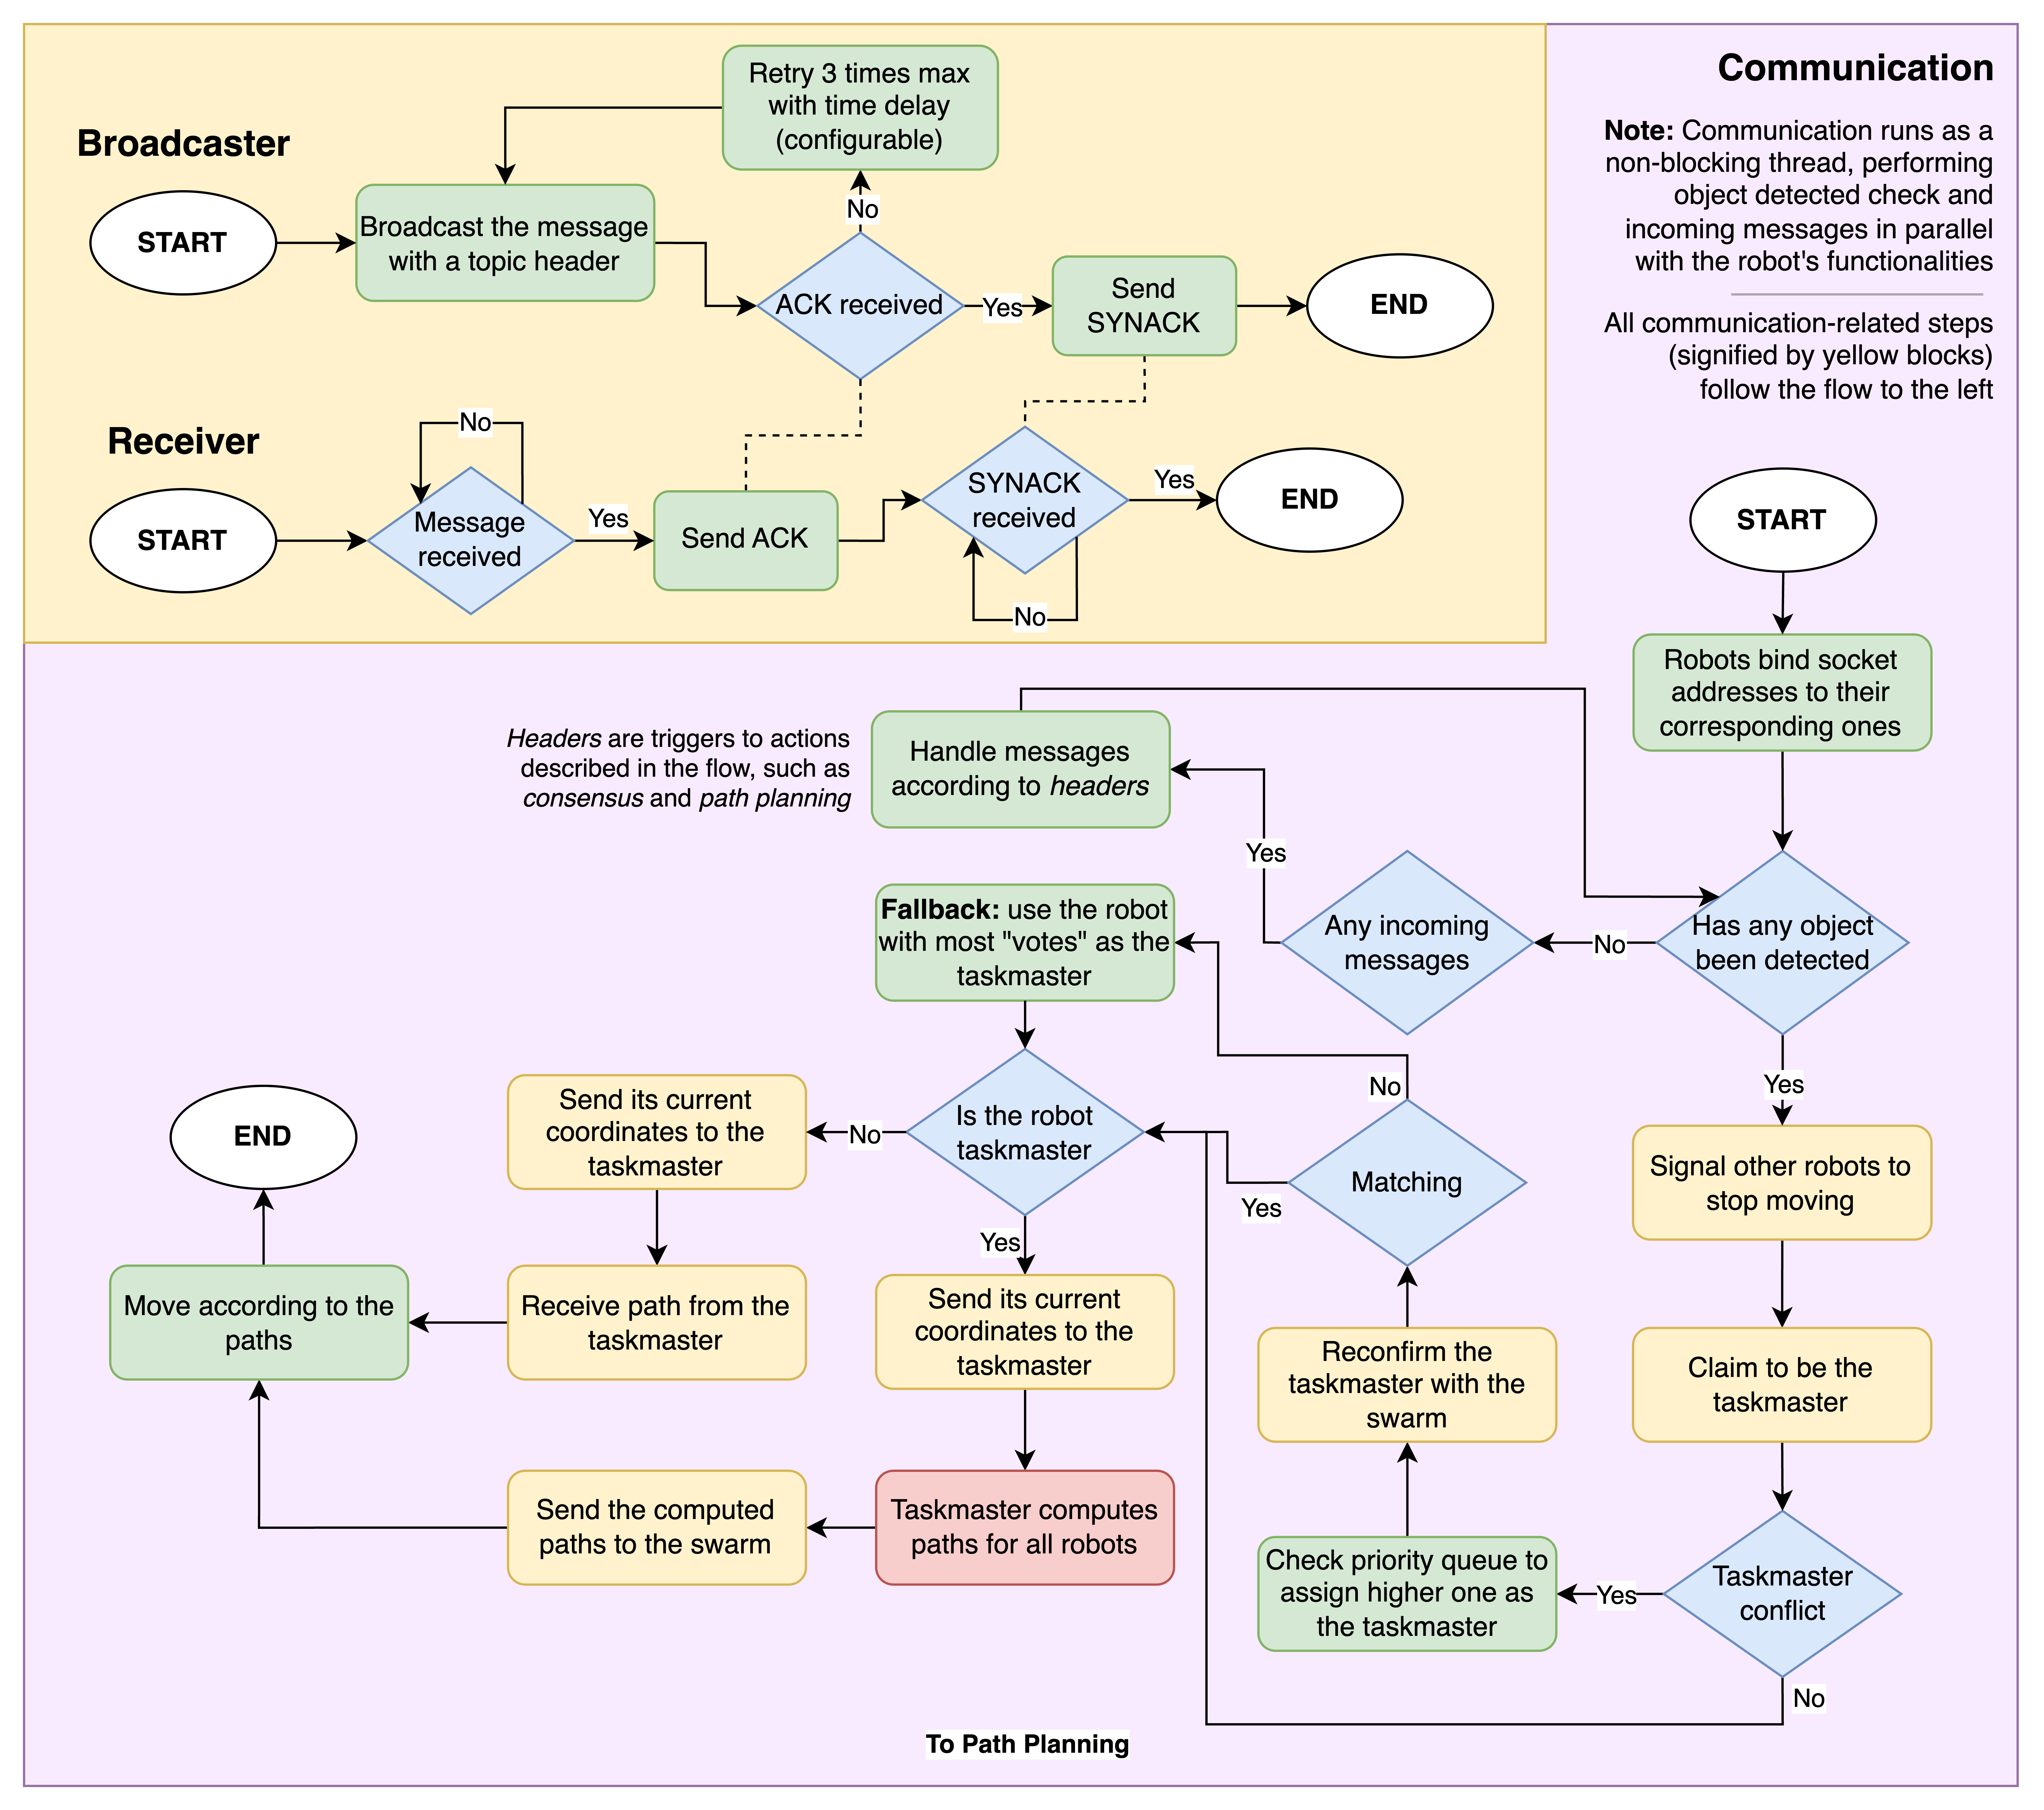
\includegraphics[width=0.85\linewidth]{assets/images/communication/communication-flow.png}
    \caption{Communication in the Swarm Detailed Flow}
    \label{fig:communication-flow}
\end{figure}


\paragraph*{}
Reliable communication is a critical component in swarm robotics, serving as a foundational element for coordinated behavior. To ensure robustness, the communication architecture was designed to incorporate a three-way handshake mechanism, similar to the approach used in the Transmission Control Protocol (TCP). This mechanism facilitates the implementation of retry logic, where message transmissions are reattempted if acknowledgments are not received within a specified timeout period, thereby enhancing the reliability of inter-robot communication.

\paragraph*{}
The general communication flow within the swarm, excluding the continuous coordinate streaming, is triggered upon the detection of a target object. When an object is identified, the detecting robot initiates a broadcast signal instructing all swarm members to temporarily halt movement. Following this, the detecting robot assumes a coordination role, computing collision-free trajectories for each member of the swarm. These planned paths are then individually assigned and transmitted to the respective robots, enabling synchronized and safe movement in accordance with the swarm’s objectives.

\paragraph*{}
Given the minimal time interval between communication and object detection, potential conflicts in signal handling must be addressed. Specifically, simultaneous detection of a target object by multiple robots may lead to multiple robots attempting to assume the role of taskmaster concurrently. To resolve such conflicts and ensure coherent swarm behavior, a consensus algorithm is employed. This algorithm leverages a predefined priority queue to determine the robot with the highest priority, which is then designated as the taskmaster. Once consensus is reached, the decision is broadcast across the swarm, and the priority queue is updated—demoting the current taskmaster to the lowest priority position. This mechanism helps to distribute leadership roles more evenly and prevent repeated taskmaster assignments to the same robot.

\paragraph*{}
Once the taskmaster has been appointed, each swarm member transmits its current coordinates to the taskmaster. These static positional data are collected while the robots remain stationary, having halted in response to the object detection signal. Using this fixed positional snapshot, the taskmaster proceeds to compute collision-free paths for the swarm. The resulting trajectories are then individually communicated back to the respective robots, enabling coordinated and efficient movement based on a consistent spatial configuration.
